\documentclass[11pt,a4paper]{article}
\usepackage[a4paper,left=1in, right=1in, top=1in, bottom=1in]{geometry}
\usepackage[latin1]{inputenc}
\usepackage{amsmath}
\usepackage{amsfonts}
\usepackage{amssymb}
\usepackage{graphicx}
\usepackage{enumitem}
\usepackage{wasysym}
\usepackage{anysize}

\usepackage{fancyhdr}
 \setlength{\headheight}{0.2in}
\pagestyle{fancy}

\lhead{\textsc{{\large The Transition to Renewable
Energy: Modeling it from the Bottom-up and the Top-Down}}}
\chead{}
\rhead{}

\lfoot{Project summary}
\cfoot{Haney, Carbajales-Dale, Heun}
\rfoot{\thepage}

\renewcommand{\headrulewidth}{0.4pt}
\renewcommand{\footrulewidth}{0.4pt}

\marginsize{1in}{1in}{0.5in}{0.5in}

\begin{document}

%\maketitle


%**** written in the third person, informative to other persons working in the same or related fields, and, insofar as possible, 
%understandable to a scientifically or technically literate lay reader.****


\section*{Overview}
\vspace*{-0.1in}

%**** activity that would result if the proposal were funded and a statement of objectives and methods to be employed. ****

The objective of this proposal is to test the hypothesis that 
interacting agents are unable to collectively manage 
a transition from non-renewable to renewable resources 
to avoid negative impacts of resource depletion. 
This research will explore the behavior of agents in 
a resource harvesting and investment `game' where 
resource managers must forage for energy and natural resources 
while investing some of those resources towards the activities of 
foraging and maintenance of vital infrastructure. 
In autonomous mode (agents act according to simple algorithms), 
advantageous strategies for resource management can be 
`evolved' through the process of `natural selection'. 
In learning mode (researchers or learners take control of the agent behavior), 
successive rounds of the game will more closely resemble real-world locations. 
Researchers can better understand the context for 
resource and infrastructure management strategies with the aim of developing improved policies.

The proposed objective will be met over the 3-year time period of the project by carrying out the following tasks:
(1)	\emph{}: 	\label{task:}
(2)	\emph{	}	\label{task:}
(3)	\emph{}: 	\label{task:}

Figure~\ref{fig:CNH_Schema}

\begin{figure}
\centering\
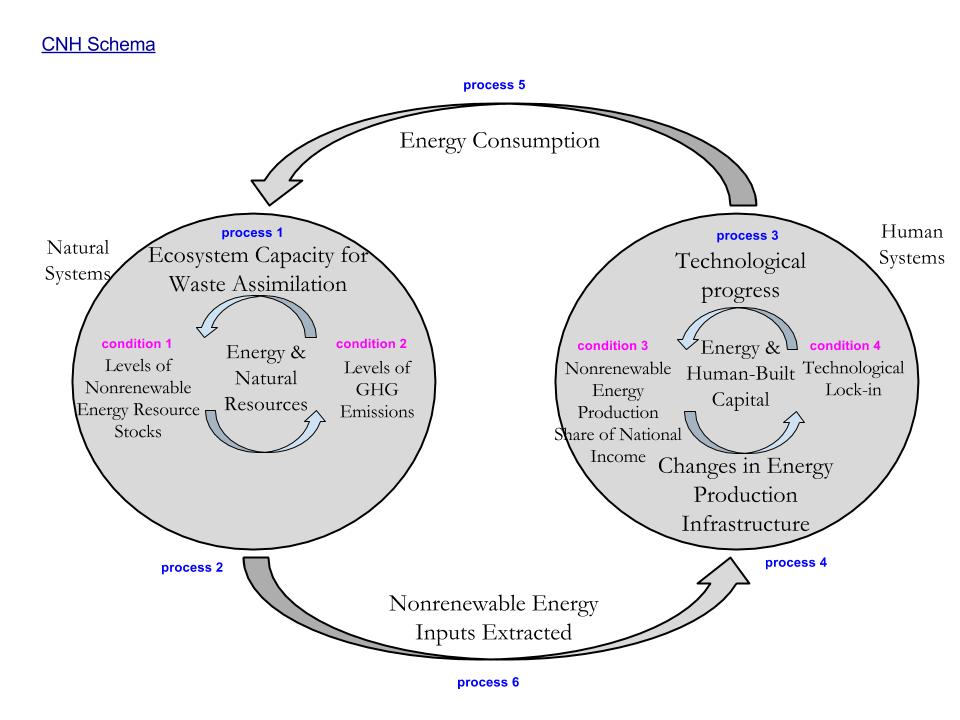
\includegraphics[width=\linewidth]{CNH_Schema.jpg}
\caption[CNH Schema]{CNH Schema for Energy Transitions.}
\label{fig:CNH_Schema}
\end{figure}
\vspace*{-0.1in}
\section*{Intellectual merit}
\vspace*{-0.1in}
%**** describe the potential of the proposed activity to advance knowledge. ****

The proposed activity will advance the current understanding of 
resource and infrastructure management and 
the conditions for successful transition from depleting resources (e.g. fossil fuels) 
to those that can be used sustainably (e.g. renewable energy). 
The novel aspect of the research is to employ techniques from social science 
to better understand resource and infrastructure management strategies.

\vspace*{-0.1in}
\section*{Broader impacts}
\vspace*{-0.1in}

%**** describe the potential of the proposed activity to benefit society and contribute to the achievement of specific, 
%desired societal outcomes.****

The `game' will identify resource and infrastructure management strategies 
to better navigate the resource transition faced by our global society. 
These strategies will be translated into recommendations for 
resource and infrastructure management and policy decision makers. 
The knowledge gained will be helpful for (especially rural and isolated) communities 
to develop strategies for sustainable resource use. 
The game will be presented as a learning tool within existing courses at Clemson 
to highlight issues of sustainability and emphasize the role of energy literacy, 
especially in currently under-served populations 
through the use of the existing programs at Clemson University.  

The long-term educational goal is to 
improve energy literacy and systems thinking 
to facilitate better-informed planning for a sustainable future. 
In pursuit of this goal, the educational objective of this proposal 
is to provide an interactive, simulated learning environment for learners 
to understand how individual behavior impacts collective opportunities 
for sustainable management of resources. 
Development of the experimental apparatus (game development) will be integrated into term projects, 
the classroom will be used as a test-bed for subsequent iterations of the game 
and to gain experimental data by having students play the game. 






\bibliography{ABM}
\bibliographystyle{unsrt}

\end{document}